% Chapter 3

\chapter{Materials} % Main chapter title

\label{Materials} % For referencing the chapter elsewhere, use \ref{Materials} 


%----------------------------------------------------------------------------------------
\section{Infectious clone of MVMp (pIC\_MVMp)}
\label{IC}


\subsection{Plasmid map of pIC\_MVMp}

\begin{figure}[h] 
\begin{center}
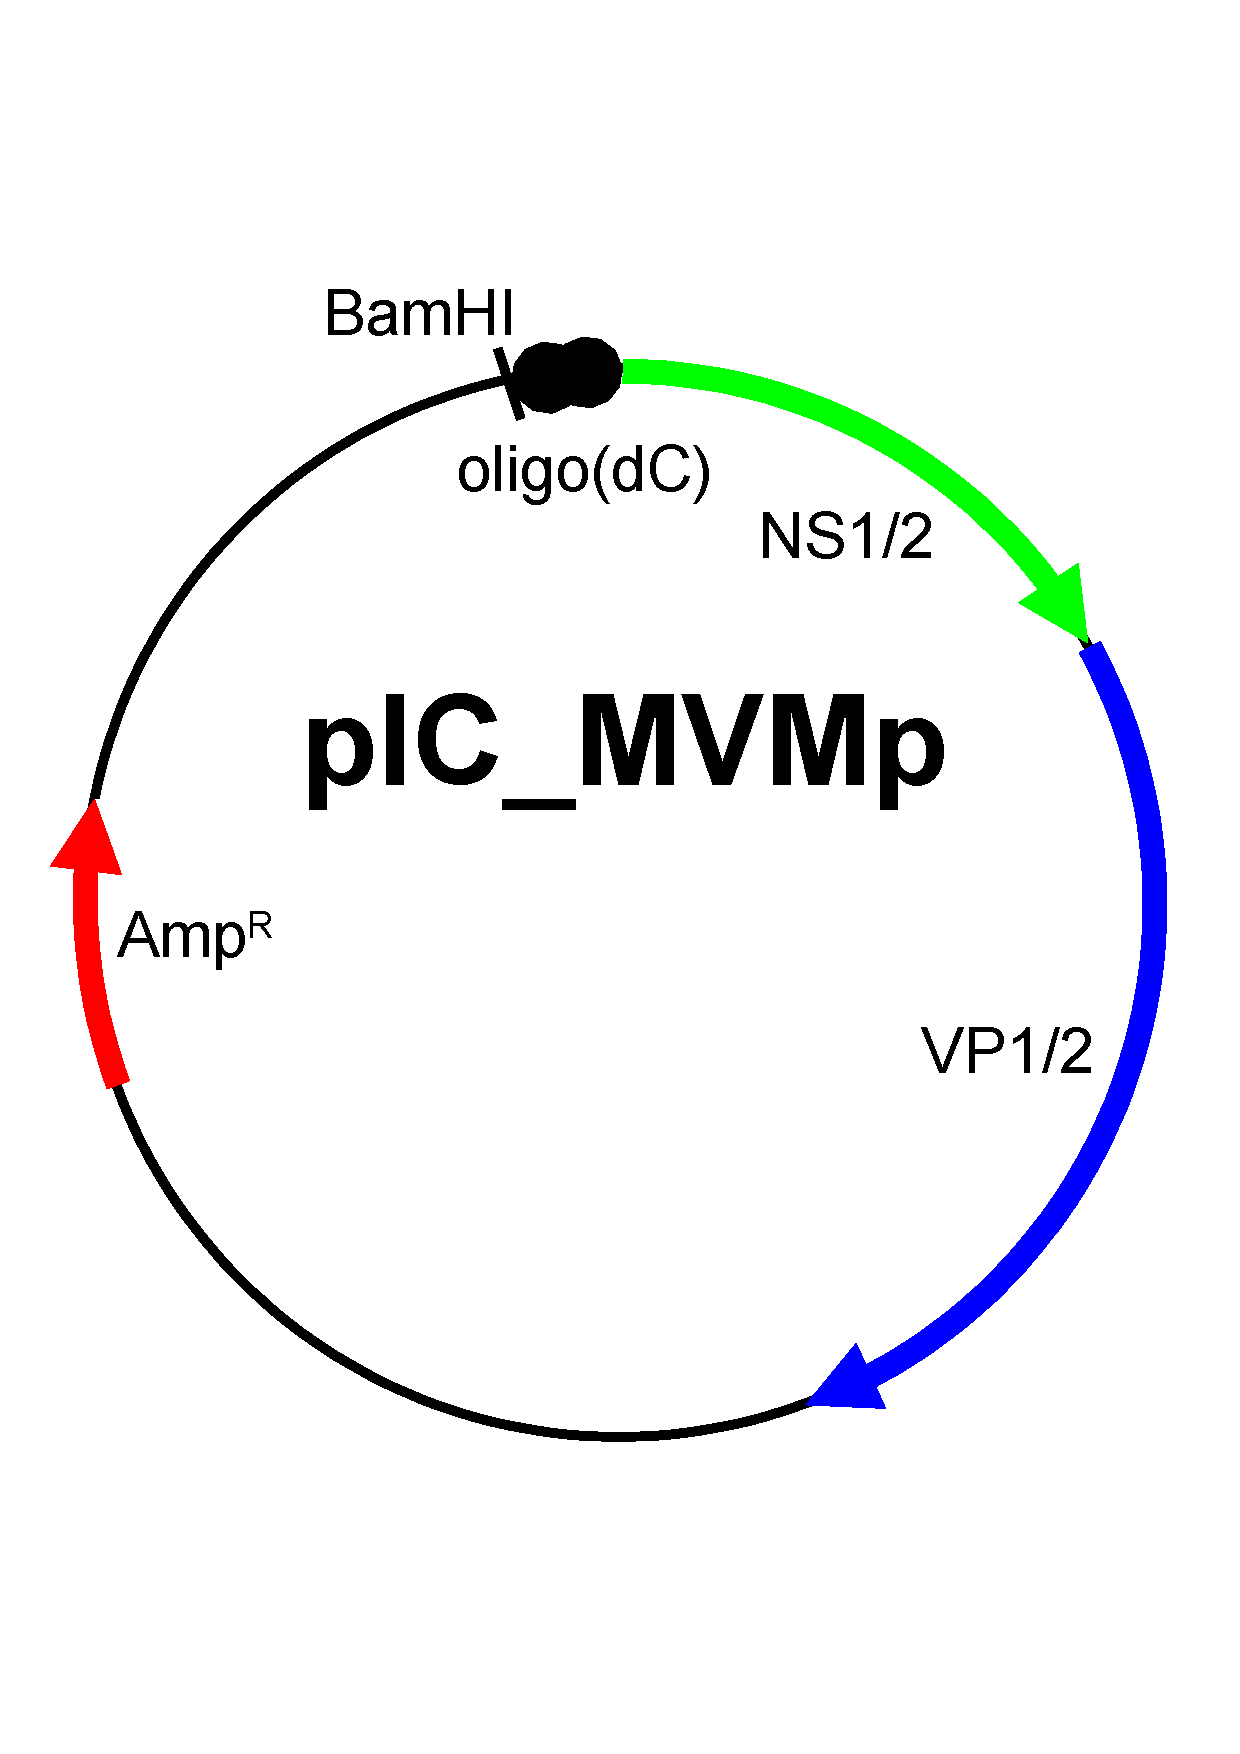
\includegraphics[width=0.65\textwidth]{pIC_MVMp}
\caption[Plasmid map of the infectious clone of MVMp]{Plasmid map of the infectious clone of MVM (pIC\_MVMp). Colored arrows indicate the genes in either the MVMp genome or the pBR322 cloning vector. The circles at the left-hand end of the MVM genome represent the oligo(dC) linker sequence which was originally used for cloning \cite{pmid6345805}.}
\label{pIC}
\end{center}
\end{figure}

\newpage

\subsection{Complete sequence of pIC\_MVMp}
\label{sequence}

\raggedright
The complete nucleotide sequence of the infectious clone of MVM (pIC\_MVMp) is shown below. Sequences in black correspond to the backbone of the pBR322 cloning vector. The sequence colored red corresponds to the viral negative (-) strand in 3' to 5' direction which is predominantly packaged into MVM capsids.  


\begin{addmargin}{0.025\textwidth}

  \begin{footnotesize}
\begin{LVerbatim}[commandchars=\\\{\}]

   1 AAGAACTTCT GCTTTCCCGG AGCACTATGC GGATAAAAAT ATCCAATTAC AGTACTATTA TTACCAAAGA
  71 ATCTGCAGTC CACCGTGAAA AGCCCCTTTA CACGCGCCTT GGGGATAAAC AAATAAAAAG ATTTATGTAA
 141 GTTTATACAT AGGCGAGTAC TCTGTTATTG GGACTATTTA CGAAGTTATT ATAACTTTTT CCTTCTCATA
 211 CTCATAAGTT GTAAAGGCAC AGCGGGAATA AGGGAAAAAA CGCCGTAAAA CGGAAGGACA AAAACGAGTG
 281 GGTCTTTGCG ACCACTTTCA TTTTCTACGA CTTCTAGTCA ACCCACGTGC TCACCCAATG TAGCTTGACC
 351 TAGAGTTGTC GCCATTCTAG GAACTCTCAA AAGCGGGGCT TCTTGCAAAA GGTTACTACT CGTGAAAATT
 421 TCAAGACGAT ACACCGCGCC ATAATAGGGC ACAACTGCGG CCCGTTCTCG TTGAGCCAGC GGCGTATGTG
 491 ATAAGAGTCT TACTGAACCA ACTCATGAGT GGTCAGTGTC TTTTCGTAGA ATGCCTACCG TACTGTCATT
 561 CTCTTAATAC GTCACGACGG TATTGGTACT CACTATTGTG ACGCCGGTTG AATGAAGACT GTTGCTAGCC
 631 TCCTGGCTTC CTCGATTGGC GAAAAAACGT GTTGTACCCC CTAGTACATT GAGCGGAACT AGCAACCCTT
 701 GGCCTCGACT TACTTCGGTA TGGTTTGCTG CTCGCACTGT GGTGCTACGG ACGTCGTTAC CGTTGTTGCA
 771 ACGCGTTTGA TAATTGACCG CTTGATGAAT GAGATCGAAG GGCCGTTGTT AATTATCTGA CCTACCTCCG
 841 CCTATTTCAA CGTCCTGGTG AAGACGCGAG CCGGGAAGGC CGACCGACCA AATAACGACT ATTTAGACCT
 911 CGGCCACTCG CACCCAGAGC GCCATAGTAA CGTCGTGACC CCGGTCTACC ATTCGGGAGG GCATAGCATC
 981 AATAGATGTG CTGCCCCTCA GTCCGTTGAT ACCTACTTGC TTTATCTGTC TAGCGACTCT ATCCACGGAG
1051 TGACTAATTC GTAACCATTG ACAGTCTGGT TCAAATGAGT ATATATGAAA TCTAACTAAA TTTTGAAGTA
1121 AAAATTAAAT TTTCCTAGAT CCACTTCTAG GAAAAACTAT TAGAGTACTG GTTTTAGGGA ATTGCACTCA
1191 AAAGCAAGGT GACTCGCAGT CTGGGGCATC TTTTCTAGTT TCCTAGAAGA ACTCTAGGAA AAAAAGACGC
1261 GCATTAGACG ACGAACGTTT GTTTTTTTGG TGGCGATGGT CGCCACCAAA CAAACGGCCT AGTTCTCGAT
1331 GGTTGAGAAA AAGGCTTCCA TTGACCGAAG TCGTCTCGCG TCTATGGTTT ATGACAGGAA GATCACATCG
1401 GCATCAATCC GGTGGTGAAG TTCTTGAGAC ATCGTGGCGG ATGTATGGAG CGAGACGATT AGGACAATGG
1471 TCACCGACGA CGGTCACCGC TATTCAGCAC AGAATGGCCC AACCTGAGTT CTGCTATCAA TGGCCTATTC
1541 CGCGTCGCCA GCCCGACTTG CCCCCCAAGC ACGTGTGTCG GGTCGAACCT CGCTTGCTGG ATGTGGCTTG
1611 ACTCTATGGA TGTCGCACTC GATACTCTTT CGCGGTGCGA AGGGCTTCCC TCTTTCCGCC TGTCCATAGG
1681 CCATTCGCCG TCCCAGCCTT GTCCTCTCGC GTGCTCCCTC GAAGGTCCCC CTTTGCGGAC CATAGAAATA
1751 TCAGGACAGC CCAAAGCGGT GGAGACTGAA CTCGCAGCTA AAAACACTAC GAGCAGTCCC CCCGCCTCGG
1821 ATACCTTTTT GCGGTCGTTG CGCCGGAAAA ATGCCAAGGA CCGGAAAACG ACCGGAAAAC GAGTGTACAA
1891 GAAAGGACGC AATAGGGGAC TAAGACACCT ATTGGCATAA TGGCGGAAAC TCACTCGACT ATGGCGAGCG
1961 GCGTCGGCTT GCTGGCTCGC GTCGCTCAGT CACTCGCTCC TTCGCCTTCT CGCGGACTAC GCCATAAAAG
2031 AGGAATGCGT AGACACGCCA TAAAGTGTGG CGTATACCAC GTGAGAGTCA TGTTAGACGA GACTACGGCG
2101 TATCAATTCG GTCATATGTG AGGCGATAGC GATGCACTGA CCCAGTACCG ACGCGGGGCT GTGGGCGGTT
2171 GTGGGCGACT GCGCGGGACT GCCCGAACAG ACGAGGGCCG TAGGCGAATG TCTGTTCGAC ACTGGCAGAG
2241 GCCCTCGACG TACACAGTCT CCAAAAGTGG CAGTAGTGGC TTTGCGCGCT CCGTCGACGC CATTTCGAGT
2311 AGTCGCACCA GCACTTCGCT AAGTGTCTAC AGACGGACAA GTAGGCGCAG GTCGAGCAAC TCAAAGAGGT
2381 CTTCGCAATT ACAGACCGAA GACTATTTCG CCCGGTACAA TTCCCGCCAA AAAAGGACAA ACCAGTGAAC
2451 TACGGAGGCA CATTCCCCCT TAAAGACAAG TACCCCCATT ACTATGGCTA CTTTGCTCTC TCCTACGAGT
2521 GCTATGCCCA ATGACTACTA CTTGTACGGG CCAATGACCT TGCAACACTC CCATTTGTTG ACCGCCATAC
2591 CTACGCCGCC CTGGTCTCTT TTTAGTGAGT CCCAGTTACG GTCGCGAAGC AATTATGTCT ACATCCACAA
2661 GGTGTCCCAT CGGTCGTCGT AGGACGCTAC GTCTAGGCCT TGTATTACCA CGTCCCGCGA CTGAAGGCGC
2731 AAAGGTCTGA AATGCTTTGT GCCTTTGGCT TCTGGTAAGT ACAACAACGA GTCCAGCGTC TGCAAAACGT
2801 CGTCGTCAGC GAAGTGCAAG CGAGCGCATA GCCACTAAGT AAGACGATTG GTCATTCCGT TGGGGCGGTC
2871 GGATCGGCCC AGGAGTTGCT GTCCTCGTGC TAGTACGCGT GGGCACCGGT CCTGGGTTGC GACGGGCTCT
2941 ACGCGGCGCA CGCCGACGAC CTCTACCGCC TGCGCTACCT ATACAAGACG GTTCCCAACC AAACGCGTAA
3011 GTGTCAAGAG GCGTTCTTAA CTAACCGAGG TTAAGAACCT CACCACTTAG GCAATCGCTC CACGGCGGCC
3081 GAAGGTAAGT CCAGCTCCAC CGGGCCGAGG TACGTGGCGC TGCGTTGCGC CCCTCCGTCT GTTCCATATC
3151 CCGCCGCGGA TGTTAGGTAC GGTTGGGCAA GGTACACGAG CGGCTCCGCC GTATTTAGCG GCACTGCTAG
3221 TCGCCAGGTC ACTAGCTTCA ATCCGACCAT TCTCGGCGCT CGCTAGGAAC TTCGACAGGG ACTACCAGCA
3291 GTAGATGGAC GGACCTGTCG TACCGGACGT TGCGCCCGTA GGGCTACGGC GGCCTTCGCT CTTCTTAGTA
3361 TTACCCCTTC CGGTAGGTCG GAGCGCAGCG CTTGCGGTCG TTCTGCATCG GGTCGCGCAG CCGGCGGTAC
3431 GGCCGCTATT ACCGGACGAA GAGCGGCTTT GCAAACCACC GCCCTGGTCA CTGCTTCCGA ACTCGCTCCC
3501 GCACGTTCTA AGGCTTATGG CGTTCGCTGT CCGGCTAGTA GCAGCGCGAG GTCGCTTTCG CCAGGAGCGG
3571 CTTTTACTGG GTCTCGCGAC GGCCGTGGAC AGGATGCTCA ACGTACTATT TCTTCTGTCA GTATTCACGC
3641 CGCTGCTATC AGTACGGGGC GCGGGTGGCC TTCCTCGACT GACCCAACTT CCGAGAGTTC CCGTAGCCAG
3711 CTGCGAGAGG GAATACGCTG AGGACGTAAT CCTTCGTCGG GTCATCATCC AACTCCGGCA ACTCGTGGCG
3781 GCGGCGTTCC TTACCACGTA CGTTCCTCTA CCGCGGGTTG TCAGGGGGCC GGTGCCCCGG ACGGTGGTAT
3851 GGGTGCGGCT TTGTTCGCGA GTACTCGGGC TTCACCGCTC GGGCTAGAAG GGGTAGCCAC TACAGCCGCT
3921 ATATCCGCGG TCGTTGGCGT GGACACCGCG GCCACTACGG CCGGTGCTAC GCAGGCCGCA TCTCCTAGGC
3991 CCCCCCCCCC CCC\color{red}AAAATCT TGACTGGTTG GTACAAGTGC ATTCACTGCA CTACTGCGCG CGACGCGCGC
\color{red}4061 GACGGAAGCC GTCAGTGTGC AGTGAATGCA AAGTGTACCA ACCAGTCAAG ATTTTTACTA TTCGCCAAGT
\color{red}4131 CCCTCAAATT TGGTTCCGCG CTTTTCCTTC ACCCGCACCA AATTTCATAT ATTCGTTGAT GACTTCAGTC
\color{red}4201 AATGAATAGA AAAGAAAGTA AGACACTCAG CTCTGCGTGT CTTTCTCTCA TTGGTTGATT GGTACCGACC
\color{red}4271 TTTACGAATG AGACTACTTC AAAACCCTCG TTGGTTGACC AATTTCCTTT TTTCATTGGT CCTTCACAAG
\color{red}4341 AGTAAACAAA AATTTTTACT TTTACAAGTT GACTTACCTT TTCTATAGCC TACCTTATCA ATGTTTTTTC
\color{red}4411 TCGACGTCCT CCTGCTCGAC TTTAGAAATG TTGCTCCTCG CCTTTGATGA ACCCTGGTTT CGCTCCTGTA
\color{red}4481 CCTTACCCTT TGGTGTCACC TACTTTACTG GTTTTTCGTT CATAAGTAAA AACTAAGAAA CCAATTTTTT
\color{red}4551 ACAAATAAAC TTCACGAATT GTGTTTCTTA TATAAAGGAC CACTACAATT AACCAAACAC GTTGTACTTA
\color{red}4621 CCCCTTTTCT GGTTCCGACC GTGACGGTAC ATGATTAACC TCCTTTCCTG AAATCAGTTC GAGTTCCCTT
\color{red}4691 TACCACCTCT TCCGTTGATT TACAAATGAC CTCGTCTACC AACCATTGTC GGACATTACA CGTTGATTGT
\color{red}4761 GGTCGACTTT CTTAATTTGA TTCTCTTTAT CGTCTTCTGT TACTCACCCA ATGAGATGAA TGAATATTCG
\color{red}4831 TATTCGTTTG GTTTTTTCTG ATATGGTTCA CACAAGAAAA ACCTTTGTAC TAACGAATGA TAAAAAATTG
\color{red}4901 ATTTTTCTTT TATTCGTGAT CAGGTGGTTC TCTGCCTCCG ATAAAAGAAA TCGTCACTGA AACCGACCTT
\color{red}4971 TTGATTGAAA AATTTTCTTC CGCTCGCGGT AGATCACTCG TTTGATATGT GACTACTGTA CGCCGGTCTT
\color{red}5041 TGCCAACTTT GGTGTCATTG GTGACGCGTC CTTTGATTCG CGCCGTCTTA AGTTTGATTT TTTCTTCAAA
\color{red}5111 GATAATTTTG ATGTGAATTT CTCGACCACG TATTTTCTCA TTGGAGTGGT CTCCTGACCT ACTACTACGT
\color{red}5181 CGGTCTGTCA ATGTAACTTT ACTACCGAGT TGGTCCACCT CTTTTGGACG ACTTTTTATG CGATCTCTAA
\color{red}5251 ACATGTGATT GAGATCGGTC TTGGTTTTGT CGTAAACTGA ATTAAAATCT TTTTCGACTT TGGTCGTTTG
\color{red}5321 ATTGGTTGAA AAGTGACGGA CTGTGTTCTT GGACGTCTTA AAAACGAAAA GTACCGACCT TGATACAATT
\color{red}5391 TCAAACGGTA CGATAAACGA CACAAAATTT GTCTGTTCCT CCGTTTTCTT TATGACAAAA TAAAGTACCT
\color{red}5461 GGTCGGTCGT GTCCGTTTAG ATAATAACGT GTTCGGTATC GTGTTCGTCA ACCGTTACAA CCAACGATAT
\color{red}5531 TACGTCGGTT ACATTTGAAA GGTAAATTAC TGACATGGTT GTTCTTGAAC TAAACCCATC TTCTTCGACC
\color{red}5601 ATTGAAACCT GTCGTTCATT TGGTCAAATT TCGGTAAACG AGACCAGTTT GATAAGCGTA ACTAGTTTTT
\color{red}5671 CCTTTTCCGT CGTTTGTCTA ACTTGGTTGT GGTCAGTAGT ACTGGTGTTT ACTCTTGTAA TGTCACCAGT
\color{red}5741 CTTATCCGAC GCTTCTTTCT GGTCTTGTGT GAGTTGGTTA GTCTCTGTCT TACGAATTGT AAGTAGATTG
\color{red}5811 TGTATGGAAC GGACCACTGA AACCAAACCA ACTGTTTTTA CTTACCGGGT ACTAAACACG AACCAACCAT
\color{red}5881 TTCTTACCAA TGGTTAGATG GTACCGTTCG ATGACACGAT TTACCCCGTT TCAAGGACTA ACCAGTCTTT
\color{red}5951 TGACCCGCCT CGGTTTCCAC GGTTGAGGAT ATTTAAATGA TCCAAGCCGT GCGAGTGGTA AGTGCTGTGG
\color{red}6021 CTTTTCATGC GGAGAGTCGG TCTTGATACG TGATTGAGGT GAACGTAGCC TAGAGCTCCT GGACCGAAAT
\color{red}6091 CTCGGAACCT CGTGTGGTTT ATGAGGACAA CGCCCGTGAC GTCTTTGGGT CTTGTGACCC CTTCGACCAA
\color{red}6161 GGTTTCGGAC GGTTCTACCA GTTGACTCGG GTTGAACCAG TCTCTAGCTC CTCCTAAACT CTCGCACGAA
\color{red}6231 GCCACGCCTT GGCAACTTCT TTCTGAAGTC GCTCGGCGAC TTGAACCTGA TTCCATGCTA CCGCGGAGGT
\color{red}6301 CGATTTTCTC GATTTTCTCC ATTCCCAAAT TCCCTACCAA CCAACCACCC CATAATTACA AATTAATGGA
\color{red}6371 CAAAATGTCC GGACTTTAGT GAACCAAAAT CCAACCCACG GAGGACCGAT GTTCATGGAC CCTGGTCCCT
\color{red}6441 TGTCGGAACT GGTTCCTCTT GGTTGGTTAG GTAGACTGCG GCGACGGTTT CTCGTGCTGC TCCGGATACT
\color{red}6511 AGTTATGTAG TTTAGACCTT TTTTAGGAAT GGACATGAAG AGACGACGAC TAGTTGCGAA ATAACTGGTT
\color{red}6581 TGGTTCCTGC GGTTTCTGAC CCCTCCGTTC CAACCAGTGA TGAAAAAATC TTGGTTCGCG CGAAAACGTG
\color{red}6651 GATTCGAACG ATGACTGAGA CTTGGACCTT GAAGACCACA TTCGTCTCGA CCATTTGCGT GATCTGGTGG
\color{red}6721 ACGAATGTAA AAATAATTGG TTCGGTCTCG ATTTTTTTTT GAATGAAGAA GACGACGTGT CGTTTCGTCA
\color{red}6791 GTTTGGTACT CACTACCGTG GTCGGTTGGA CTGTCGCCTT TGCGACAGGT GAGTCGACGT TCTCAACTTG
\color{red}6861 CTCGTCGACT GCCGGGACCT CCGAGACCCC CACCCCCGAG ACCGCCCCCA CCCCAACCAC AAAGATGACC
\color{red}6931 CAGAATACTA TTAGTTTGCG TAATATCTAA GAACCCACTG CCGACCCATC TTTAATGACG TGATCGTTGA
\color{red}7001 TCTGATCATG TAAATTTGTA CGGATTTAGT CTTTTGATAA CGTCTTAGTC TCAAGTGTTA TGTTGTCTGT
\color{red}7071 GTAGTCAGTT TCCGTTGTAC CGTTTTCTAC TACGAGTACT CGTTTAAACC TGTGGTACCT CGAACCACCT
\color{red}7141 ACGATTACGA ACCCCTCAAA CCGAGGTCGG TTCACTGACC GTTATGTAAA CGTTGTGGTA CTCGGTCGAA
\color{red}7211 TTGAACCATA GTGAACTAGT TCTTTATAAG TTACATCACG ACTTTTGACA ATGTCTCGTT CTGAATCCTC
\color{red}7281 CAGTTCGATA TTTTTATATG TTGTTACTGG AATGTCGAAC GTACTACCAA CGTCATCTGA GTTTGTTGTA
\color{red}7351 AAACGGTATG TGTGGACGTC GTTTGAGTTA CCTTTGTGAA CCAAAGATGG GGACCTTTGG TTGGTATCGT
\color{red}7421 AGTGGTATGT CCATGATAAA AACGCAACTG TCTCTAGAAA GTCACTGGAT GCTTTTAGTT CTTCCGTGTC
\color{red}7491 AACTTGTATT ACACTACCCT TGTGGTTTTC CTTACTTAAG AGTTAAAAAA TGGTAACTCT TGTGTGTTGT
\color{red}7561 TTAGTGTAAC GAGTCTTGTC CCCTGCTTAA ACGGTGTCCG TGAATGATGA AACTGTGTTT AGGTCAATTT
\color{red}7631 GAGTGTGTGT GCACCGTTTG GTTGGCAGTT GAACCTGTCG GAGGTGACGA CAGTTGGAAA GGACTTCGAC
\color{red}7701 TGTGACTACG TCCATGTGAA TGACGAGTTC CCTCGTCTGT ACCTTGTTGT GTTTACCCCC AATTGACCCA
\color{red}7771 CTCACTTCGT TAGTCTTGGT CTGGACGAGT TCATCCTAAA ACAGTTGGTG TGGTACTGAA ACTTCGGTCG
\color{red}7841 TCTCGACCTG GTAAACGACG GGGTTTTCAA GGTCGTCTAT AATGAGTTCC TCATCTGTTT CTTCGGTTAC
\color{red}7911 CGTCACAATC TATGTCAATA CCGTTTGTCG TACCACTTTT AACCCGAAGT GTACCTGGTC GTGGTCTCGC
\color{red}7981 GATGTGTACC CTACTTTGTT CGAAACCAAG TCCATCTCTG TGGTTTCTAC CAAAATAAGT TAGTCGTGGT
\color{red}8051 GATCAACAAG GTGGTGGTGA TTTACCGTAA GAATGTTTAC GTTTGGGATA ACCCTGATTT TTACTGTAAG
\color{red}8121 TAAAAAGTTT ACAAAAATTG TCGATACCAG GTGATTGACG TAAAAGTGTG GGTTCAGGAC ATATGGGAGT
\color{red}8191 TCCTGTTTAT ACCCTGTTTC TTGATCTAGA ACTTGTGTTT GGATCTGAAG TGTATTGACG AGGTAAACAA
\color{red}8261 ACATTTTTGT TACGTGGACC TGTTTACAAC CAATCTAATC CTGGTTTGGA TTGACTGGTT ATACTAGGTT
\color{red}8331 TGCCTCGGTG TGAAAGATCT TAACAATGTA TACCATGTAA AAAGACCTTT CCTTTTGATT GGTACTCTCG
\color{red}8401 TTTTGAATCT CGATTGTGGT GAACCTTGGG TCACATGGTT CATTCACGAC TTCTGTTACC GTTGAGTATG
\color{red}8471 TACTCACATT GATTTACCGA TGGTTGACGA TGACCTTTGT ACGTCAGACA CGGCGAATAT TGTTCTGGAC
\color{red}8541 AACGATCTTT ATGAATGATT GATTGGTACG AAAAAGAAAG ACATGAAGTA TATAATAATT CTGATTATTT
\color{red}8611 CTATGTTGTA TCTTTATATT ATAATGTATA TCTAAATTCT TTATCTTATT ATACCATGAA TCATTGACAA
\color{red}8681 TTTTTATTAT CTTGGAAACC TTATTGTTCT ATCAATCAAC CAATTACAAT CTATCTTATT CTTCTAGTAC
\color{red}8751 ATATTACTTA TTTTCCCACC TTCCCACCAA CCATCCAATT ACAATCTATC TTATTCTTCT AGTACATATT
\color{red}8821 ACTTATTTTC CCACCTTCCC ACCAACCATC CATAAGGGAA TCTGAACTAC AATTCCTGGT TTTTTTATTA
\color{red}8891 TTTTGAAAAA ATTTTGAGTT GGTTCTGATG ACAGATAAGT CACTTGGTTG ACTTGGTAAT CATAATGATA
\color{red}8961 CAAAAATCCC ACCCT\color{black}CCAGT TAGTTAGTCC TT 
\end{LVerbatim}
\end{footnotesize}

\end{addmargin}

\newpage




\section{Chemicals and compounds}

\begin{center}

\begin{longtable}{l l}
\textbf{Chemical} & \textbf{Provider}\\
\hline
\endfirsthead

\multicolumn{2}{l}{\textbf{Table~\ref{Chemicals}} continued}\\
\\
\textbf{Chemical} & \textbf{Provider}\\
\hline
\endhead

Acetic Acid (Glacial) & Merck\\
Acetone & Merck\\
Agarose low EEO & Applichem\\
Ampicillin (Ready Made Solution, 100 g/mL, 0.2
$\mu M$   
filtered)& Sigma-Aldrich\\
Bafilomycin A\textsubscript{1} & Sigma-Aldrich \\
Bovine Serum Albumin (BSA) & Sigma-Aldrich\\
Bromophenol Blue & Merck\\
Caesium Chloride (CsCl) & Sigma-Aldrich\\
Chymostatin & Sigma-Aldrich\\
Citric Acid & Sigma-Aldrich\\
Complete Mini Protease Inhibitor Cocktail Tablets & Roche \\
Complete Mini Protease Inhibitor Cocktail Tablets EDTA-free & Roche \\
1,4-diazabicyclo[2.2.2]octane (DABCO) & Sigma-Aldrich\\
4',6-diamidino-2-phenylindole (DAPI) & Invitrogen \\
Dimethyl Sulfoxide (DMSO) & Sigma-Aldrich \\
Dithiothreitol (DTT) & Sigma-Aldrich\\
1kb DNA Ladder & Invitrogen \\
Ethylenediaminetetraacetic Acid (EDTA) & Sigma-Aldrich \\
Ethanol (99.89 \%) & Sigma-Aldrich \\
Ethanol (94 \%) denat. with 2 \% MEK & Grogg Chemie AG\\
Ethidium Bromide (10 mg/mL) & Invitrogen \\
EZMix\textsuperscript{\texttrademark} N-Z-Amine\textsuperscript{\textregistered} A (NZ Amine) & Sigma-Aldrich \\
Fetal Calf Serum (FCS) & Amimed \\
Glycerol (Anhydrous) & Sigma-Aldrich \\
Goat Serum & DAKO \\
G-Protein Agarose Beads & Santa Cruz Biotech \\
Hydrochloric Acid (HCl) & Sigma-Aldrich \\
Imidazole & Sigma-Aldrich\\
Iminodiacetic Acid & Sigma-Aldrich\\
Isopropanyl $\beta$-D-1-thiogalactopyranoside (IPTG) & Invitrogen \\
LB-Agar, Miller & Sigma-Aldrich\\
LB Broth Base & Invitrogen\\
L-Glutamine (200 mM) & Biochrom \\
Magnesium Chloride (MgCl\textsubscript{2}) & Sigma-Aldrich \\
Magnesium Sulfate (MgSO\textsubscript{4}) & Sigma-Aldrich \\
Manganese(\RM{2}) chloride (MnCl\textsubscript{2}) & Sigma-Aldrich\\
2-Mercaptoethanol & Sigma-Aldrich \\
Methanol HPLC grade & Fisher Chemical \\
Milk Powder (Adapta) & Coop \\
Mowiol & Calbiochem \\
Nitrocellulose Transfer Membranes 0.45 $\mu$m & Millipore \\
2-(\textit{N}-morpholino)ethanesulfonic acid (MES) & Sigma-Aldrich\\
3-(\textit{N}-morpholino)propanesulfonic acid (MOPS) & Sigma-Aldrich\\
Nonidet P40 (NP-40) & Applichem \\
NuPage MOPS SDS-Running Buffer (20$\times$) & Invitrogen\\
Nupage Transfer Buffer (20$\times$) & Invitrogen \\
N-Z-Amine\textsuperscript{\textregistered} A & Sigma-Aldrich \\
Penicillin/Streptomycin & Biochrom AG \\
Phosphate-Buffered-Saline (PBS) & Oxoid \\
Polybuffer\textsuperscript{\textregistered} 74 & Sigma-Aldrich \\
Precision Plus Protein Standards, Dual Color & BioRad \\
Sodium Acetate, anhydrous & Sigma-Aldrich\\
Sodium Citrate & Sigma-Aldrich\\
Sodium Chloride (NaCl) & Roth \\
Sodium dihydrogen phosphate Dihydrate (NaH\textsubscript{2}PO\textsubscript{4}$\cdot$2H\textsubscript{2}O) & Sigma-Aldrich\\
Sodium dodecyl sulfate (SDS) & Sigma-Aldrich\\
di-Sodium hydrogen phosphate Dihydrate (Na\textsubscript{2}HPO\textsubscript{4}$\cdot$2H\textsubscript{2}O) & Sigma-Aldrich\\
Sodium Fluoride (NaF) & Sigma-Aldrich\\
Sodium Hydroxide (NaOH) & Sigma-Aldrich \\
Sodium Orthovanadate (Na\textsubscript{3}VO\textsubscript{4}) & ICN Biomedicals Inc.\\ 
D(+)-Sucrose & Sigma-Aldrich \\
Sulfuric Acid 95-98 \% & Sigma-Aldrich\\
Tris(hydroxymethyl)aminoethane (Tris Buffer) & Sigma-Aldrich \\
Triton X-100 & Siegfried \\
Tween 20 & Applichem \\
Yeast Extract & Sigma-Aldrich \\

\caption[Chemicals and compounds]{List of chemicals and compounds}\\

\label{Chemicals}
\end{longtable}

\end{center}



\section{Buffers}

\subsection{General buffers}

\begin{table}[H]
\begin{tabular}{l l r}
\textbf{Buffer} & \textbf{Reagent} & \textbf{Concentration}\\
\hline
\\
Cell Lysis Buffer & Tris-HCl (pH 7.2) & 50 mM\\ & NaCl & 150 mM \\ & Nonidet P40 (NP-40) & 1 \% (v/v) \\ & EDTA & 5 mM\\ & Sodium orthovanadate (Na\textsubscript{3}VO\textsubscript{4}) & 1 mM\\ & Sodium fluoride (NaF) & 1 mM\\ & Protease Inhibitor Cocktail & 1 tablet per 10 mL \\ [0.3 cm] 
Nuclei Lysis Buffer & Tris-HCl (pH 7.2) & 50 mM\\ & NaCl & 150 mM\\ & Triton X-100 & 1 \% (v/v)\\ & EDTA & 5 mM\\ & Sodium orthovanadate (Na\textsubscript{3}VO\textsubscript{4}) & 1 mM\\ & Sodium fluoride (NaF) & 1 mM\\ & Protease Inhibitor Cocktail & 1 tablett per 10 mL\\ [0.3 cm]
Phosphate Buffered Saline & PBS Tablets & 1 tablet in 100 mL \\ 
(PBS Buffer) & & dH\textsubscript{2}O\\ [0.3 cm]
Phosphate Buffered Saline with & PBS Buffer & \\
Bovine Serum Albumin & Bovine Serum Albumin (BSA) & 1\% (w/v) in PBS \\
(PBSA Buffer) & & \\ [0.5 cm]

\end{tabular}

\caption[General buffers]{Buffers used for cell lysis and standard incubations.}
\label{General buffers}
\end{table}

\subsection{Chromatography buffers}
\subsubsection{Anion-exchange chromatography (AEX)}

\begin{center}
\begin{table}[H]
\begin{tabular}{l l r}
\textbf{Buffer} & \textbf{Reagent} & \textbf{Concentration}\\
\hline
\\
Sample Buffer & Tris-HCl (pH 8) & 10 mM\\
& EDTA & 1 mM\\
& Sodium orthovanadate (Na\textsubscript{3}VO\textsubscript{4}) & 1 mM\\
& Sodium fluoride (NaF) & 1 mM\\ [0.3 cm]

Starting Buffer & Tris-HCl (pH 7.2) & 20 mM\\ 
& EDTA & 1 mM\\ [0.3 cm]

Elution Buffer & Tris-HCl (pH 7.2) & 20 mM\\
& EDTA & 1 mM\\
& NaCl & 2 M\\ [0.5 cm] 
\end{tabular}
\caption[Anion-exchange chromatography (AEX) buffers]{Buffers used for anion-exchange chromatography (AEX).}
\label{AEX buffers}
\end{table}

\end{center}


\subsubsection{Chromatofocusing (CF)}

\begin{center}
\begin{table}[H]
\begin{tabular}{l l r}
\textbf{Buffer} & \textbf{Reagent} & \textbf{Concentration}\\
\hline
\\
Buffer A & Bis-Tris (pH 7, adjusted with saturated iminodiacetic acid) & 25 mM\\ [0.3 cm]
Buffer B & Polybuffer 74 (pH 4, adjusted with saturated iminodiacetic acid) & 20 \% in ddH\textsubscript{2}O\\ [0.5 cm]
\end{tabular}
\caption[Chromatofocusing (CF) buffers]{Buffers used for chromatofocusing (CF).}
\label{CF buffers}
\end{table}

\end{center}

\subsection{Agarose gel electrophoresis}

\begin{table}[H]
\begin{tabular}{l l r}
\textbf{Buffer} & \textbf{Reagent} & \textbf{Concentration}\\
\hline
\\
6$\times$ DNA Loading Buffer & D(+)-Sucrose & 40 \% (w/v) \\
& Bromophenol blue & 0.25 \% (w/v)\\ [0.3 cm]

10$\times$ Tris-Acetate-EDTA Buffer & Tris base (pH 8.0) & 400 mM \\
(TAE Buffer) & Acetic acid (glacial) & 11.5 \% (v/v) \\
& EDTA & 10 mM \\ [0.5 cm]

\end{tabular}
\caption[Agarose gel electrophoresis buffers]{Buffers used for agarose gel electrophoresis.}
\label{Gel electrophoresis}
\end{table}


\subsection{Western blot}

\begin{table}[H]
\begin{tabular}{l l r}
\textbf{Buffer} & \textbf{Reagent} & \textbf{Concentration}\\
\hline
\\
1$\times$ NuPage MOPS Buffer & \multicolumn{2}{p{8cm}}{20$\times$ buffer was diluted to 1$\times$ with dH\textsubscript{2}O and used for SDS page.} \\ [0.3 cm]

1$\times$ NuPage Transfer Buffer & \multicolumn{2}{p{8cm}}{20$\times$ buffer was diluted to 1$\times$ with 20 \% methanol. This Buffer was used to transfer the separated proteins to the nitrocellulose membrane.} \\ [0.3 cm] 

2$\times$ Protein Loading Buffer (PLB) & Tris-HCl (pH 6.8) & 120 mM \\
(non-reducing, \cite{pmid5432063}) & Sodium dodecyl sulfate (SDS) & 4 \% (w/v)\\
& Glycerol & 20 \% (v/v) \\
& Bromophenol blue & 0.02 \% (w/v)\\ [0.3 cm]

10$\times$ Tris-Buffered Saline & Tris-HCl (pH 7.3) & 0.2 M \\
(TBS Buffer) & NaCl & 1.5 M \\ [0.3 cm]

1$\times$ Tris-Buffered Saline with Tween 20 & 10$\times$ TBS & 10 \% (v/v) \\
(TBST Buffer) & Tween 20 & 0.05 \% (v/v)\\ [0.5 cm]

\end{tabular}

\caption[Western blot buffers]{Buffers used for Western blotting analysis.}
\label{Western blot}
\end{table}




\section{Kits}

\begin{center}

\begin{table}[H]
\begin{tabular}{l l}
\textbf{Ready-to-use Reaction System (Kit)} & \textbf{Provider}\\
\hline
\\
Amaxa\textsuperscript{\texttrademark} Cell Line Nucleofector\textsuperscript{\texttrademark} Kit R & Lonza Group AG\\
Amaxa\textsuperscript{\texttrademark} Cell Line Nucleofector\textsuperscript{\texttrademark} Kit V & Lonza Group AG\\
Amersham Hyperfilm\textsuperscript{\texttrademark} ECL & GE Healthcare\\
Carestream\textsuperscript{\textregistered} Kodak\textsuperscript{\textregistered} autoradiography GBX developer/replenisher & Sigma-Aldrich\\
Carestream\textsuperscript{\textregistered} Kodak\textsuperscript{\textregistered} autoradiography GBX fixer/replenisher & Sigma-Aldrich\\
DNeasy Blood and Tissue Kit & Qiagen\\
Dynabeads\textsuperscript{\textregistered} mRNA DIRECT\textsuperscript{\texttrademark} Kit & Invitrogen\\
iTaq\textsuperscript{\texttrademark} Universal SYBR\textsuperscript{\textregistered} Green Supermix & BioRad\\
Nuclei EZ Prep Kit & Sigma-Aldrich\\
pBluescript \RM{2} KS(+) Phagemid Kit & Agilent Technologies\\
QIAEX \RM{2}\textsuperscript{\textregistered} Gel Extraction Kit & Qiagen\\
QIAGEN Plasmid Midi Kit & Qiagen\\
QIAprep\textsuperscript{\textregistered} Spin Miniprep Kit & Qiagen\\
QIAquick\textsuperscript{\textregistered} PCR Purification Kit & Qiagen\\
QuikChange\textsuperscript{\textregistered} Site-Directed Mutagenesis Kit & Agilent Technologies\\
SuperSignal\textsuperscript{\textregistered} West Femto Maximum Sensitivity Substrate & Thermo Scientific\\
XL-10 Ultracompetent Cells & Agilent Technologies\\
\\
\end{tabular}

\caption[Ready-to-use Reaction Systems (Kits)]{Ready-to-use kits.}
\label{Kits}
\end{table}
\end{center}


\section{Enzymes}

\begin{center}

\begin{longtable}[H]{l r p{1cm} l}
\textbf{Enzyme} & \multicolumn{2}{c}{\textbf{Concentration}} & \textbf{Provider}\\
\hline
\\
$\alpha$-Chymotrypsin & 10 & mg/mL & Sigma-Aldrich \\
DNaseI, RNase free & \np{10000} & U/mL & Roche \\
Neuraminidase & \np{50000} & U/mL & New England Biolabs \\
$\lambda$-Phosphatase & \np{400000} & U/mL & Merck \\
Trypsin/EDTA solution & \multicolumn{2}{l}{0.25 \% / 0.02 \% (w/v)} & Biochrom AG \\
\\

\caption[Enzymes]{The listed enzymes were used for \textit{in vitro} treatments or passing tissue culture cells.}
\label{Enzymes}
\end{longtable}

\end{center}


\section{Antibodies}
\subsection{Primary antibodies}

\begin{small}
\begin{center}
\begin{table}[H]
\begin{tabular}{ P{2 cm} p{4.5cm} l l P{2.3 cm} p{3 cm}}
\textbf{Name} & \textbf{Specificity} & \textbf{Host} & \textbf{Clonality} & \textbf{Dilution} & \textbf{Provider}\\
\hline
\\
$\alpha$-VP (Jimmy) & Linear epitopes on VP1 and VP2 of MVM. & Rabbit & Polyclonal & IF: 1/800 WB: 1/\np{2000}  & J. M. Almendral \cite{pmid15367635}\\ [0.3 cm] 

$\alpha$-Caps \newline(B7) & Conformational surface epitope on intact capsids of MVM. & Mouse & Monoclonal & IF: 1/100 & J. M. Almendral \cite{pmid12552010} \\ [0.3 cm] 

%Early Endosome Marker (EEA1, ab2900) & Detects a band at 180 kDa that represents EEA1 in WB \cite{pmid7768953}. & Rabbit & Polyclonal & IF: 1/300 & Abcam \\ 
%Late Endosome Marker (ab2733) & Epitope in the extracellular domain of M6PR. & Mouse & Monoclonal & IF: 1/300 & Abcam \\ 
%Lysosome Marker (LAMP-1) &  Both LAMP-1 and LAMP-2 are involved in maintaining lysosome acidity and protecting the lysosomal membranes from autodigestion, and their expression is increased in patients with lysosomal storage disorders. & Mouse & Monoclonal & IF: 1/300 & Santa Cruz Biotechnology Inc. \\
N-VP2 & N-terminal part of VP2. & Rabbit & Polyclonal & IF: 1/200 WB: 1/\np{1000} & J. M. Almendral \cite{pmid15367635}\\ [0.5 cm]

\end{tabular}

\caption[Primary antibodies]{\normalsize The primary antibodies were used for immunolabeling, immunoprecipitation, and Western blotting analysis.}
\label{Primary antibodies}
\end{table}
\end{center}
\end{small}


\subsection{Secondary antibodies}

\begin{footnotesize}

\begin{center}
\begin{table}[H]
\begin{tabulary}{1\textwidth}{ P{3.4 cm} p{1.5 cm} l p{3 cm} P{2.3 cm} p{3 cm}}
\textbf{Name} & \textbf{Target species } & \textbf{Host} & \textbf{Conjugate} & \textbf{Dilution} & \textbf{Provider}\\
\hline
\\
Goat $\alpha$-mouse IgG & Mouse & Goat & Alexa Fluor\textsuperscript{\textregistered}~488 & IF: 1/500 & Life Technologies \\[0.3 cm]

Goat $\alpha$-mouse IgG & Mouse & Goat & Alexa Fluor\textsuperscript{\textregistered}~594 & IF: 1/500 & Life Technologies \\[0.3 cm]

Goat $\alpha$-mouse Ig & Mouse & Goat & Horseradish peroxidase (HRP) & WB: 1/\np{20000} & Dako \\[0.3 cm]

Goat $\alpha$-rabbit Ig & Rabbit & Goat & Horseradish peroxidase (HRP) & WB: 1/\np{20000} & Dako \\[0.3 cm]

Goat $\alpha$-rabbit IgG & Rabbit & Goat & Alexa Fluor\textsuperscript{\textregistered}~488 & IF: 1/500 & Life Technologies \\[0.3 cm]

Goat $\alpha$-rabbit IgG & Rabbit & Goat & Alexa Fluor\textsuperscript{\textregistered}~594 & IF: 1/500 & Life Technologies\\[0.5 cm]

\hline \\
\multicolumn{6}{l}{\normalsize All secondary antibodies listed in this table are polyclonal.} \\[0.5 cm]
\end{tabulary}

\caption[Secondary antibodies]{The secondary antibodies were used for immunofluorescence assays and Western blotting analysis.}
\label{Secondary antibodies}
\end{table}
\end{center}
\end{footnotesize}





\nomenclature{Ig}{Immunoglobulin}



\section{Media} 

\begin{center}
\begin{table}[H]
\begin{tabular}{l l}
\textbf{Name} & \textbf{Provider}\\
\hline
\\
Dulbecco's Modified Eagle Medium (DMEM) & Gibco\\
Lysogeny Broth Agar (LB Agar) & Sigma-Aldrich\\
Lysogeny Broth Medium (LB Medium) & Sigma-Aldrich\\
SOC Medium & Sigma-Aldrich\\ [0.5 cm]
\end{tabular}
\caption[Media]{The denoted media were used for the cultivation of A9 and NB324K cells, as well as XL1-blue and XL10-gold bacteria.}
\label{Media}
\end{table}
\end{center}